%%%% CAPÍTULO 2 - REVISÃO DA LITERATURA (OU REVISÃO BIBLIOGRÁFICA, ESTADO DA ARTE, ESTADO DO CONHECIMENTO)
%%
%% O autor deve registrar seu conhecimento sobre a literatura básica do assunto, discutindo e comentando a informação já publicada.
%% A revisão deve ser apresentada, preferencialmente, em ordem cronológica e por blocos de assunto, procurando mostrar a evolução do tema.
%% Título e rótulo de capítulo (rótulos não devem conter caracteres especiais, acentuados ou cedilha)
\chapter{Referencial te\'orico}\label{cap:referencialTeorico}

Neste trabalho, o objetivo foi desenvolver um multímetro capaz de medir tensão e corrente simultaneamente e enviar os dados para um smartphone por meio de uma conexão wifi. Considerando essa proposta, foram analisadas duas opções para servir como base: um multimedidor e um multímetro.

O multimedidor é um dispositivo geralmente trifásico, que permite a medição simultânea de tensão e corrente, exibindo as formas de onda em um display. Possui três ou mais canais simultâneos. No entanto, apresenta a limitação de possuir apenas um referencial de medição, com resolução na ordem de 1V nos modelos mais baratos e 0,1V nos modelos mais caros, repetindo-se esses valores para a resolução da corrente [CITAÇÃO].

Por outro lado, o multímetro é um dispositivo monofásico que permite a medição de apenas um canal por vez, como tensão, corrente, resistência, capacitância, entre outros. Ele não exibe as curvas na tela, fornecendo apenas os valores. A resolução varia, sendo que nos modelos mais simples pode chegar a 0,1 mV, enquanto a resolução da corrente é da ordem de 1uA [CITAÇÃO].

Considerando que o dispositivo deve ser utilizado como uma ferramenta didática em sala de aula, é essencial que a resolução seja adequada para o bom aproveitamento das disciplinas. Além disso, a apresentação das formas de onda também é relevante. Assim, optou-se por uma abordagem que combina características de ambos os dispositivos, utilizando os diagramas de blocos para identificar as funcionalidades e suas relações com o dispositivo a ser produzido.

Para o multimedidor, foi utilizado o diagrama de blocos do \textit{oZm3}, um produto \textit{open source} (projeto aberto) já introduzido no mercado, sendo uma versão trifásica de outro, também \textit{open source} chamado \textit{(openZmeter)}. Ambos possuem interface de apresentação dos dados via uma página do navegador de um celular ou computador.

\begin{figure}[h]
    \caption{Diagrama de blocos do multimedidor trifásico oZm3}
    \label{fig:ozm3flowchart}
    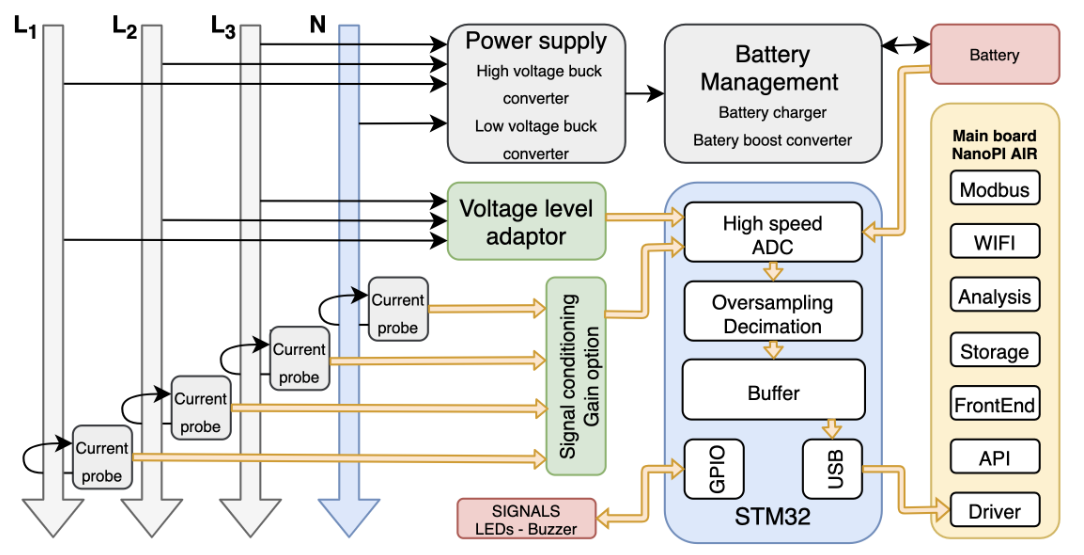
\includegraphics[width=0.8\textwidth]{figuras/openzmeter-diagrama.png}
    \fonte{CITAR Open Source Oz3.pdf}
\end{figure}

Para o multímetro, foi utilizado um diagrama de blocos disponível no site da (CITAÇÃO) \autoref{fig:ozm3flowchart} \textit{Texas Instruments}, que explica o funcionamento de um produto completo.

\begin{figure}[h]%% Ambiente figure
    %\captionsetup{width=0.55\textwidth}%% Largura da legenda
    \caption{Exemplo de um Diagrama de Blocos de um Multímetro}%% Legenda
    \label{fig:multimeterflowchart}%% Rótulo
    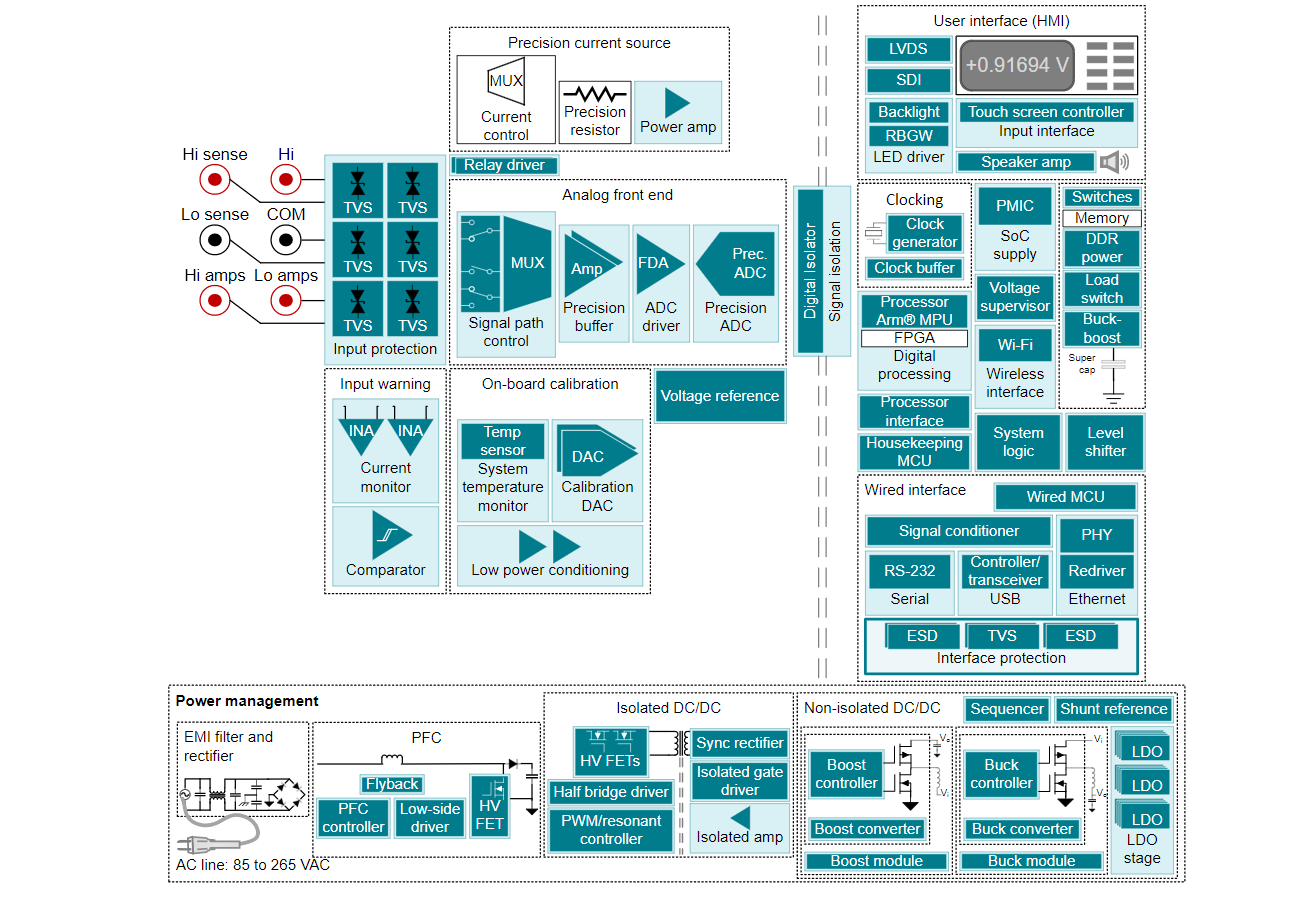
\includegraphics[width=1\textwidth]{flowchart}%% Dimensões e localização
    \fonte{Texas Instruments}%% Fonte
\end{figure}

% RAFAEL --------------------------------------------------------------------------------------------------------

\section{Diagrama de Blocos}\label{sec:fchart}

Como premissa de organização, para melhor apresentar os tópicos envolvidos, será utilizado o diagrama de blocos de um multimetro com o design feito pela Texas Instruments como guia base.

\begin{figure}[htb]%% Ambiente figure
    %\captionsetup{width=0.55\textwidth}%% Largura da legenda
    \caption{Exemplo de um Diagrama de Blocos de um Multímetro}%% Legenda
    \label{fig:flowChart2}%% Rótulo
    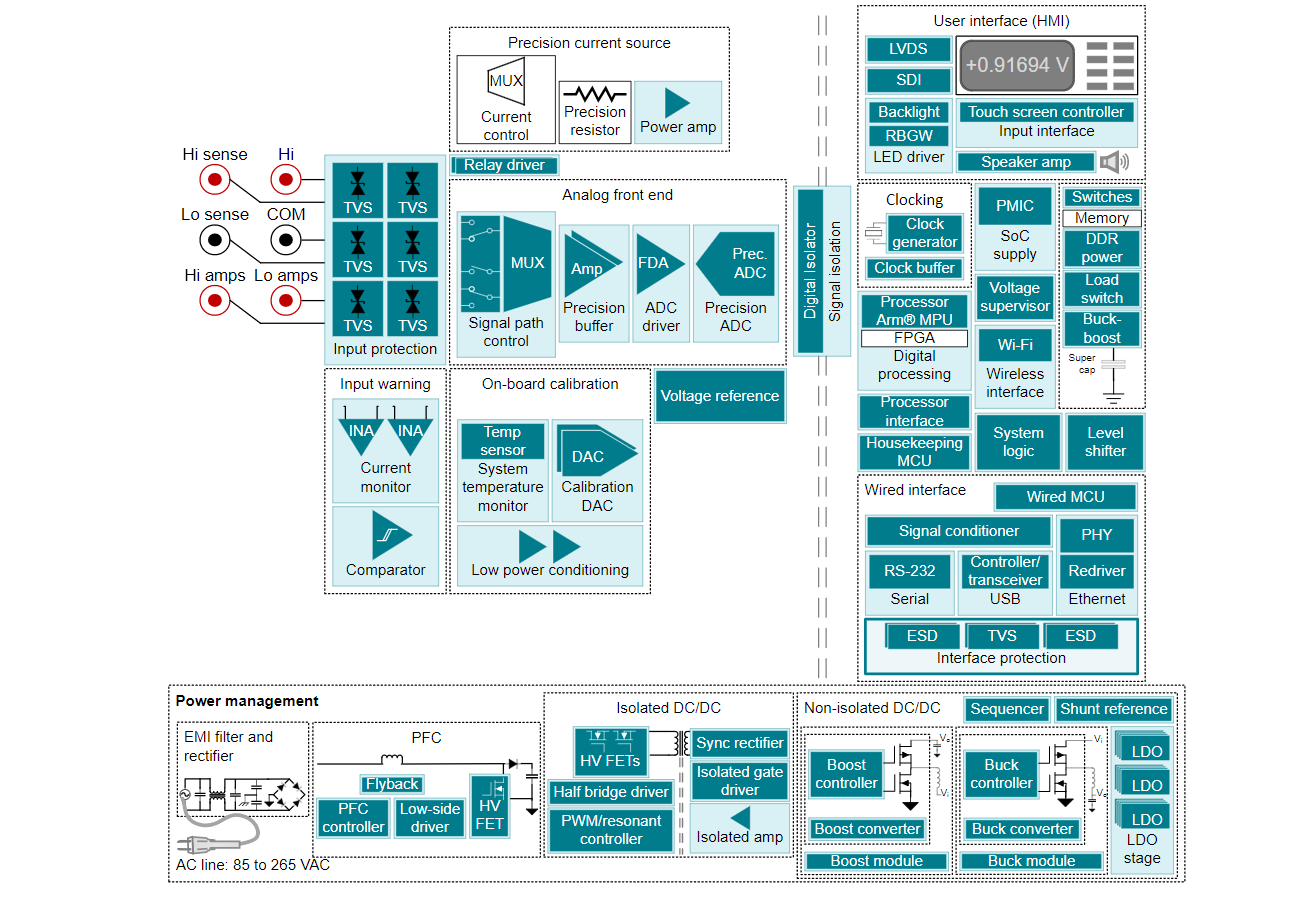
\includegraphics[scale=0.4]{flowchart}%% Dimensões e localização
    \fonte{Texas Instruments}%% Fonte
\end{figure}

\section{Proteção de Entrada}\label{sec:InputProtection}

Proteção de entrada é um assunto extremamente abrangente quando se trata de circuitos eletrônicos. Dependendo da função que este tenha que exercer, existem infinitas topografias que podem ser consideradas. Algumas exigências, porém, são comuns, como a necessidade de um circuito de proteção contra descargas eletrostáticas, ou ESD (Electrostatic Discharge). Tais descargas podem entregar picos de tensão extremamente altos, chegando até a 30 kV, o que é extremamente danoso a qualquer circuito que use semicondutores. Pulsos de pico tão alto quanto 2500 V já são o suficiente para danificar a maioria dos circuitos eletrônicos. Notóriamente, seres humanos são capazes de entregar descargas de até 20 kV porcausa da capacitância inata à sua fisiologia %%citar o documento http://www.reallyreallyrandom.com/zener/media/Zener_Theory_and_Design.pdf, página 65



\subsection{ESD}\label{subsec:electrostaticDischarge}

Esse tipo de proteção é necessária para circuitos que fazem interface com o meio físico e normalmente é exercida por um circuito básico de TVS (Transient Voltage Supressor). Estes circuitos, também chamados de circuitos de clamping, reagem a transientes (ou picos) de tensão, fechando um curto entre o circuito e o ground do equipamento, dissipando assim tal anomalia.

\section{Calibração}\label{sec:OpenLoopCalibration}

\section{Referência de Tensão}\label{sec:VoltageReference}

\section{Conversor Analógico Digital}\label{sec:ADC}

\subsection{Condicionamento de Sinal}\label{sec:SignalConditioning}


% ANDREY------------------------------------------------------------------------

\section{Aquisição de Sinal}\label{sec:aqSignal}

    \subsection{Monofásica e Monocanal}\label{subsec:aqSMono}

    \subsection{Trifásica e Multicanal}\label{subsec:aqSMulti}

\section{Aviso de Entrada Incorreta \textit{(Input Warning)}}\label{sec:inpWarning}

    \subsection{Monofásico e Monocanal}\label{subsec:inpWMono}

    \subsection{Trifásico e Multicanal}\label{subsec:inpWMulti}

\section{Isolador de sinal digital \textit{(Digital Signal Isolator)}}\label{sec:DSIsolator}

\section{MCU e Interface de Comunição}\label{sec:MCUInterface}

    \subsection{Microcontroladores}\label{subsec:MCU}

    \subsection{Interface de Comunicação}\label{sec:Interface}